\chapter{Writing Load Objects}

Load objects carry out the database manipulation originating from
one record from a data stream. A load object groups together all database
manipulations required for a separate selfcontained record from a
data stream. As such all the database manipulations either fail (rollback\index{rollback})
or succeed (commit\index{commit}). It is important to notice that
a LO is completely self contained. Its only connection to the outside
world is the model file (which is implicit) and the LO\_keys. These
are in fact the fields that constitute the data stream under consideration.
Being selfcontained and parameterized from the outside the load object
can either be called from a batch\index{Datastream!batch} program
or an interactive GUI program\index{Datastream!GUI}. 

In case some of the business rules are violated, the transaction is
aborted and rolled back (in case some database modifications were
already done). The errors are returned in a data structure of its
own and leave it processing to the calling program. In batch processing
the errors are written into the appropriate database tables, GUIs
usually have to shown the errors in the form immediately.

One function of the load objects is the relate error to the fields
that held the data. These are usually the keys in the LO\_keys. However,
for the reference fileds of the model file, e.g. db\_animal, db\_code, db\_address, this may
become quite involved. Consider the database column db\_animal. This
is the internal animal number after translation from the outside external
identifications to the internal. In particular, db\_animal is a function
of db\_unit which in turn is derived from CLASS / EXT\_code. This
means that db\_animal depends on three external identifications. In
this case all three may get marked as being the culprit.


\section{The pseudo SQL code, general syntax}

The connection between the source data fields and the checking in
the business rules layer (well hidden in the routine meta\_db which
is called in the load object) is derived from the pseudo SQL code
used for database modifications in the LO. Up to now select, insert
and update statements could be used with these pseudo SQL syntax.
The example in table \ref{pseudoSQL} implies an insert of a record
in table MYTABLE with the columns animal\_nr, weight, and weigh\_dt.
The values for the three columns are taken from the perl variables
\$animal\_nr, \$weight, and \$measure\_dt. It is a requirement that
these source variables are part of the data input hash LO\_keys to
the LO. Typically, they will come from the outside world (outside
the LO) either from INSPOOL records for batch programs or the GUI
fields for GUI programs. These keys are also used in the error hash
(for description see \ref{errorhash})to collect any errors that may
occur during execution of the business rules.

Sometimes data elements are also generated in the LO itself. This
may be the case in the processing of birth records in pigs, where
individual piglet identifications are generated on the basis of number
of piglets born (see LO\_DS02 for an example). Here, we would have
additional source variables that are not part of the input hash LO\_hash.
If this variable is to be used in the pseudo SQL code and must be
added to the hash LO\_keys. Only then can the error processing code
the 'culprit' i.e. the source variable responsible for the error (should
there be an error).

%
\begin{table}[htbp]

\caption{\label{pseudoSQL}the pseudo SQL in the load objects}

\begin{lyxcode}
\$pseudo\_sql{[}0{]}=~(

~~~~~~~'INSERT~into~MYTABLE~(

~~~~~~~~~~~~~~~~animal\_nr,~~weight,~~~weigh\_dt

~~~~~~~)VALUES~(

~~~~~~~~~~~~~~~\$animal\_nr,~\$weight,~\$measure\_dt)'

);\end{lyxcode}

\end{table}


In the following we will discuss the load object LO\_DS01.pm\index{Load Object!LO\_DS01.pm}
with the matching DS01.pm\index{Datastream!DS01.pm} as it is used
in batch processing.


\section{The pseudo SQL code with ENCODING}

The APIIS design feature to disconnect the outside coding from it
internal representation, while providing flexibility for future changes,
does require additional action during database access. This action
is the required translation of any external coding into internal codes
used throughout the database. There are two ways to deal with this
translation. Firstly, in the LO the programmer can retrieve the internal
codes by using standard DBI accesses to the database and then use
the retrieved internal codes in the pseudo SQL code. While it provides
flexibility, it does require error handling which can be avoided by
using the second mechanism.

Here, when the model file contains in the CONSTRAINTS section of a table the expression REF\_COL:column\_name1 then only the external codes must be used and not internal ones. The situation is the same when we have in the CHECK section of a column ForeignKey rule that leads in the end to reference column. If this is used, the BR layer
must only contain external codes and not internal ones. There is one important exception from this rule: when we want to insert a new animal in transfer, new code in table codes, i.e. new internal identificator, we have to supply the internal number as shown in the following example:
\begin{verbatim}
my $db_animal2=$apiis->DataBase->seq_next_val('seq_transfer__db_animal');
	 $data_hash{db_animal2} = $db_animal2;

         # generate new piglet numbers:
         $data_hash{piglet} = $data_hash{dam_hb_nr} . '|' . $notch;

         $pseudo_sql_2[0] =
            'INSERT INTO transfer (
                    db_animal,
                    ext_animal,
                    db_unit,
                    opening_dt,
                    entry_dt,
                    db_entry_action
            ) VALUES (
                    $db_animal2,
                    $piglet ["start_notch_no, born_alive_no"] ,
                    concat( "society|sex", $dam_society."|2" ),
                    $today[],
                    $today[],
                    "birth"
	    )' ;
\end{verbatim} 


\section{The error hash\label{errorhash}}

The generell structure of the error hash is described in the library
Apiis::Errors. The predefined keywords and structure is shown in Table
\ref{cap:Structure-of-error}.

%
\begin{table}[htbp]

\caption{Structure of error hash\label{cap:Structure-of-error}}

\begin{lyxcode}
{\footnotesize my~@type\_values~=~qw/~DATA~DB~OS~PARSE~CODE~PARAM~CONFIG~UNKNOWN~/;~}{\footnotesize \par}

{\footnotesize \#~Error~types:~}{\footnotesize \par}

{\footnotesize \#~DATA~the~passed~data~is~not~ok~(usually~in~CheckRules)~~~~~~~~~~~~~~~~}{\footnotesize \par}

{\footnotesize \#~DB~errors~from~the~database~(e.g.~unique~index~violation)~}{\footnotesize \par}

{\footnotesize \#~OS~errors~from~the~operation~system~(e.g.~full~hard~disk)~}{\footnotesize \par}

{\footnotesize \#~PARSE~errors~in~ParsePseudoSQL~with~parsing~pseudo~SQL~code~}{\footnotesize \par}

{\footnotesize \#~CODE~programming~errors,~e.g.~from~applications~like~load~objects~}{\footnotesize \par}

{\footnotesize \#~PARAM~passed~parameter~is~wrong~or~missing~}{\footnotesize \par}

{\footnotesize \#~CONFIG~one~of~the~configuration~files~is~wrong~or~has~missing~entries~}{\footnotesize \par}

{\footnotesize \#~UNKNOWN~is~unknown~:\textasciicircum{})}{\footnotesize \par}

{\footnotesize my~@severity\_values~=~qw/~FATAL~NON-FATAL~/;~}{\footnotesize \par}

{\footnotesize my~@action\_values~=~qw/~INSERT~UPDATE~DELETE~SELECT~DECODE~ENCODE~UNKNOWN~/;}{\footnotesize \par}

{\footnotesize \#~structure~of~error~messages:}{\footnotesize \par}

{\footnotesize my~\%struct;~tie~\%struct,~'Tie::IxHash';}{\footnotesize \par}

{\footnotesize \%struct~=~(~type~=>~undef,~\#~predefined~values~above~}{\footnotesize \par}

~{\footnotesize ~~~~~~~severity~=>~undef,~\#~predefined~values~above~}{\footnotesize \par}

~{\footnotesize ~~~~~~~~~action~=>~undef,~\#~predefined~values~above}{\footnotesize \par}

~{\footnotesize ~~~~~~~~~~~from~=>~undef,~\#~location~where~this~error~comes~from~(e.g.~sub,~rule)~}{\footnotesize \par}

~{\footnotesize ~~~~~~record\_id~=>~undef,~\#~id~of~this~record,~e.g.~record\_seq~from~inspool}{\footnotesize \par}

~{\footnotesize ~~~~~~~~~~~unit~=>~undef,~\#~unit~that~provides~this~data}{\footnotesize \par}

~{\footnotesize ~~~~~~~db\_table~=>~undef,~\#~database~table~concerned}{\footnotesize \par}

~{\footnotesize ~~~~~~db\_column~=>~undef,~\#~database~column~concerned}{\footnotesize \par}

~{\footnotesize ~~~~~~~~~~~data~=>~undef,~\#~just~handled~incorrect~data}{\footnotesize \par}

~{\footnotesize ~~~~~~~ext\_cols~=>~undef,~\#~involved~external~columns~(array)}{\footnotesize \par}

~{\footnotesize ~~~~~~~~~~~~~ds~=>~undef,~\#~data~stream~name}{\footnotesize \par}

~{\footnotesize ~~~~~~~err\_code~=>~undef,~\#~coded~error~message}{\footnotesize \par}

~{\footnotesize ~~~~~~msg\_short~=>~undef,~\#~main~error~message~for~end~users}{\footnotesize \par}

~{\footnotesize ~~~~~~~msg\_long~=>~undef,~\#~detailed~error~message}{\footnotesize \par}

~{\footnotesize ~~~~~~~~~~misc1~=>~undef,~\#~user~defined~scalar}{\footnotesize \par}

~{\footnotesize ~~~~~~~~~~misc2~=>~undef,~\#~user~defined~scalar}{\footnotesize \par}

~{\footnotesize ~~~~~~misc\_arr1~=>~undef,~\#~user~defined~array}{\footnotesize \par}

~{\footnotesize ~~~~~~misc\_arr2~=>~undef,~\#~user~defined~array}{\footnotesize \par}

~{\footnotesize ~~~~~~~~~);~}\end{lyxcode}

\end{table}



\section{An example: The Load Object LO\_DS01\index{Load Object!LO\_DS01}}

The simple load object LD\_DS01 performs the database actions related
with a new insemination record. In this example it needs to do:

\begin{enumerate}
\item Insert new record into SERVICE\index{table!SERVICE} 
\item Update last action (la\_rep) in ANIMAL\index{table!ANIMAL}
\end{enumerate}
%
\begin{table}[htbp]

\caption{\texttt{\small LO\_DS01.pm\label{tab:LO-DS01.pm}\index{Load Object!LO\_DS01.pm}}}

\texttt{\small ~ 1 \#\#\#\#\#\#\#\#\#\#\#\#\#\#\#\#\#\#\#\#\#\#\#\#\#\#\#\#\#\#\#\#\#\#\#\#\#\#\#\#\#\#\#\#\#\#\#\#\#\#\#\#\#\#\#\#\#\#\#\#\#\#\#\#\#\#\#\#\#}{\small \par}

\texttt{\small ~ 2 \# \$Id: actual\_docu.lyx,v 1.37 2003/12/15 13:54:40
eg Exp \$}{\small \par}

\texttt{\small ~ 3 \# This is the Load Object for a new insemination
record.}{\small \par}

\texttt{\small ~ 4 \# It is responsible to:}{\small \par}

\texttt{\small ~ 5 \#~~~~~~~~~~ 1. Insert new record into
SERVICE}{\small \par}

\texttt{\small ~ 6 \#~~~~~~~~~~ 2. Update last action (la\_rep)
in ANIMAL}{\small \par}

\texttt{\small ~ 7 \#\#\#\#\#\#\#\#\#\#\#\#\#\#\#\#\#\#\#\#\#\#\#\#\#\#\#\#\#\#\#\#\#\#\#\#\#\#\#\#\#\#\#\#\#\#\#\#\#\#\#\#\#\#\#\#\#\#\#\#\#\#\#\#\#\#\#\#\#}{\small \par}

\texttt{\small ~ 8 sub LO\_DS01 \{}{\small \par}

\texttt{\small ~ 9~~~ my \%data\_hash = \%\{ shift () \};}{\small \par}

\texttt{\small ~10~~~ }{\small \par}

\texttt{\small ~11 }{\small \par}

\texttt{\small ~12~~~ \# These are the required LO\_keys for DS01.pm:}{\small \par}

\texttt{\small ~13~~~ my @LO\_keys = qw( dam\_hb\_nr dam\_society
dam\_breed sire\_hb\_nr}{\small \par}

\texttt{\small ~14~~~~~ sire\_society sire\_breed service\_dt
);}{\small \par}

\texttt{\small ~15 }{\small \par}

\texttt{\small ~16~~~ \# some basic checks:}{\small \par}

\texttt{\small ~17~~~ my ( \$err\_status, \$err\_ref ) = CheckLO(
\textbackslash{}\%data\_hash, \textbackslash{}@LO\_keys );}{\small \par}

\texttt{\small ~18~~~ return ( \$err\_status, \$err\_ref ) if
\$err\_status;}{\small \par}

\texttt{\small ~19 }{\small \par}

\texttt{\small ~20~~~ my @pseudo\_sql;}{\small \par}

\texttt{\small ~21~~~ \$pseudo\_sql{[}0{]} = (}{\small \par}

\texttt{\small ~22~~~~~~ 'INSERT into service (}{\small \par}

\texttt{\small ~23~~~~~~~~~~ db\_animal,}{\small \par}

\texttt{\small ~24~~~~~~~~~~ db\_sire,}{\small \par}

\texttt{\small ~25~~~~~~~~~~ service\_dt,}{\small \par}

\texttt{\small ~26~~~~~~~~~~ db\_service\_typ}{\small \par}

\texttt{\small ~27~~~~~~ ) VALUES (}{\small \par}

\texttt{\small ~28~~~~~~~~~~ concat( \char`\"{}society|sex\char`\"{},
\$dam\_society.\char`\"{}|2\char`\"{}, \$dam\_hb\_nr ),}{\small \par}

\texttt{\small ~29~~~~~~~~~~ concat( \char`\"{}society|sex\char`\"{},
\$sire\_society.\char`\"{}|1\char`\"{}, \$sire\_hb\_nr ),}{\small \par}

\texttt{\small ~30~~~~~~~~~~ \$service\_dt,}{\small \par}

\texttt{\small ~31~~~~~~~~~~ \char`\"{}insem\char`\"{})'}{\small \par}

\texttt{\small ~32~~~ );}{\small \par}

\texttt{\small ~33 }{\small \par}

\texttt{\small ~34~~~ \$pseudo\_sql{[}1{]} = (}{\small \par}

\texttt{\small ~35~~~~~~ 'UPDATE animal SET}{\small \par}

\texttt{\small ~36~~~~~~~~ la\_rep~~~ = \char`\"{}SERVICE\char`\"{},}{\small \par}

\texttt{\small ~37~~~~~~~~ la\_rep\_dt = \$service\_dt}{\small \par}

\texttt{\small ~38~~~~~~~~ where db\_animal = concat( \char`\"{}society|sex\char`\"{},
\$dam\_society.\char`\"{}|2\char`\"{}, \$dam\_hb\_nr )'}{\small \par}

\texttt{\small ~39~~~ );}{\small \par}

\texttt{\small ~40 }{\small \par}

\texttt{\small ~41~~~ \$apiis->DataBase->dbh->commit;~~~ \# clean start of transaction}{\small \par}

\texttt{\small ~42~~~ \$hash\_ref = meta\_db( \textbackslash{}@pseudo\_sql,
\textbackslash{}\%data\_hash );}{\small \par}

\texttt{\small ~43~~~ \$hash\_ref->\{err\_status\} ? \$apiis->DataBase->dbh->rollback
: \$apiis->DataBase->dbh->commit;}{\small \par}

\texttt{\small ~44~~~ return ( \$hash\_ref->\{err\_status\}, \$hash\_ref->\{err\_ref\}
);}{\small \par}

\texttt{\small ~45 \}}{\small \par}

\texttt{\small ~46 }{\small \par}

\texttt{\small ~47 1;}
\end{table}


\begin{lyxlist}{00.00.0000}
\item [lines~9~--~10:]The input parameters are passed from DS01 (or
from a GUI\_DS01) (via subroutine \texttt{\scriptsize Process\_LO\_Batch}).
Some data streams need the reporting unit for their processing, others
(like LO\_DS01) can simply ignore it.
\item [lines~13~--~14:]This defines the names of the external data fields
which have to be used by any program that sends data to this load
object. (Actually, LO\_keys is a sufficient set of information to
run the Load Object. It needs to be derived directly from the data
streams that should have been described before.)
\item [lines~17~--~18:]CheckLO test the accordance of LO\_keys with
the keys of the \%data\_hash.
\item [lines~20~--~39:]A SQL-like description language is used to pass
the parameters to the subsequent processing. This PseudoSQL is described
in section .
\item [line~41:]A commit\index{database!commit} to the database is executed
to start this transaction with a well defined status.
\item [line~42:]All needed parameters (PseudoSQL and the data hash) are
passed to the subroutine meta\_db() which prepares and executes the
database actions.
\item [line~43:]Depending of the return status of meta\_db() the transaction
is committed or rolled back\index{database!rollback}.
\item [line~44:]The load object returns either success (\$err\_status
= 0) or an error status $>$ 0 and the accompanied error messages.
\end{lyxlist}

\subsection{Passing parameters with PseudoSQL\label{section:PseudoSQL}\index{Load Object!PseudoSQL}}

To pass the parameters to the subroutine meta\_db() for database transactions
it was decided to choose a SQL-like syntax. This description language
is parsed later to extract the important variables and data. These
are the rules for parsing PseudoSQL: 

\begin{itemize}
\item The Pseudo-SQL-Statements must be surrounded by \textbf{single} quotation
marks. No substitution of the Perl variables should take place. PseudoSQL
is only an artificial language to pass the parameters. Strings inside
these statements must be framed by \textbf{double} quotation marks.
\\
Example: \texttt{\small \$pseudo\_sql{[}0{]} = 'INSERT into litter
( db\_animal, delivery\_dt, comment ) VALUES ( \$dam\_hb\_nr, \$delivery\_dt,
\char`\"{}this is a comment\char`\"{} );} 
\item To concatenate values you can use the key word 'concat'. The single
elements of this concatenation must be separated by commas. Fixed
strings and variables can be mixed. The Perl concatenation operator
. can also be used. \\
Example: \texttt{\small concat( \char`\"{}society|sex\char`\"{}, \$dam\_society
. \char`\"{}|2\char`\"{}, \$dam\_hb\_nr )}{\small \par}
\item Variables, whose names do not point to an external field of the incoming
data stream can be assigned external names in brackets. The names
in brackets \textbf{must} be surrounded by double quotation marks
in total, not every single element. \\
Examples: \texttt{\small \$piglet{[}\char`\"{}start\_notch\_no, born\_alive\_no\char`\"{}{]}
concat(\char`\"{}society|sex\char`\"{}, \$dam\_society .\char`\"{}|2\char`\"{},
\$piglet{[}\char`\"{}start\_notch\_no, born\_alive\_no\char`\"{}{]})} 
\item Do you use a variable that does not point to any external field you
have to supply this variable with empty brackets. \\
Example: \texttt{\small \$today{[}{]}}{\small \par}
\item All variables, that you use in the Pseudo-SQL-Statements have to appear
as a key (without the dollar character \$) in the \%data\_hash which
you pass to meta\_db(). Usually this will be the (already existing)
field names of the incoming data. You have to add variables which
newly appear in the load object like \$piglet, \$today, \$now or also
the separately passed external unit \$ext\_unit. Just have a look
into LO\_DS02.pm for some examples.
\end{itemize}

\section{Calling a Load Object and some other issues}

As stated above a load object needs to get its input values (i.e.
the data elements defined for that particular data stream) from a
calling program. There are two modes how this can be done: input comes
from a batch program, i.e. data are read from a file or data are entered
via a GUI\index{GUI} program. A description of the former is to be
found in the inspool section of this document. GUI programs on the
other hand can be created automatically by the program mkLOform which
may be called as: \texttt{mkLOform LO\_{*} '\$PDBL\_LOCAL/model/apiis.model'}
\index{mkLOform}. As output it creates for each matching load object
one GUI program. What happens is that mkLOform picks up the LO\_key\index{key}
line from the load object which holds all elements defined for the
data stream. Then it creates for each of these elements one GUI field.
The GUI program can be run right away allowing the user to enter data
into the fields and sending them to the load object by pressing the
insert button. From there on the load object takes over doing all
the database interactions defined under the control of the business
rules.

The fields in the GUI program can be moved around the canvas using
the FormDesigner \index{FormDesigner}to suit the artistic and ergonomic
requirements of the user.

Sometimes data need to be derived from individual data. One example
is the individual recording of piglet weight at birth from which we
may want to derived the total number born, the sum of males and female
piglets and the total litter weight at birth (while this implies redundancy
we still may want to do it). To generate these sums in a Perl code
is very easy, thus doing this in the load object is a piece of cake.
However, there is the problem of not knowing in advance how many piglet
a litter has. One way of approaching this problem would be to have
one record for the sow and birthdate and the one for each piglet.
This has a number of problems: firstly, the complete set of information,
i.e. all the records pertaining to one litter constitute a transaction.
If we split this up into separate database activities, we cannot roll
the already entered data back should a later database action require
this. Secondly, one litter plus the piglet information are infact
a unit that the person entering the data would like to see as one
block. Thus, it would be desirable to have the GUI form start with
the block on the sow and then have one line for each piglet. Thus,
we would need to have enough space for a litter, 20 lines should be
ok. Then after the last piglet has been entered the complete form
content will be processed by the load object and do the necessary
accumulations on those variables that are not undef. The program mkLOform
\index{mkLOform} will then again generate the GUI program. Because
it places all fields below each other FormDesigner\index{FormDesigner}
will have to be used to arrange the fields in a more meaningful way.

This little paragraph reflect the progress made since the last one
was written. Because we are essentially lazy people Hartmut has meanwhile
rewritten mkLOform\index{mkLOfrm} into mkLOfForm\index{mkLOfForm} 
formatted forms from load objects) which produces GUI programs
on the basis of the LO\_Keys from the load objects that does multiple
fields per line. This is simply done by arranging the entries in the
LO\_Keys as is desired in the GUI program. An example is given in
table \ref{cap:Arrangement-of-keys}. The arrangement given will result
in a GUI program with 5 lines. The first would be one field with ext\_unit,
the second line would hold the three fields dam\_hb\_nr, dam\_society
and dam\_breed. The program is given in figure \ref{cap:GUI-program-automatically}.

%
\begin{table}[htbp]

\caption{\label{cap:Arrangement-of-keys}Arrangement of keys for the GUI program}

\begin{lyxcode}
~{\scriptsize ~~my~@LO\_keys~=~qw~(~}{\scriptsize \par}

~{\scriptsize ~~~~~~~~~~~~~~~~~~~~ext\_unit~~~~~~~~~~~~~~~~~~~~~~~}{\scriptsize \par}

~{\scriptsize ~~~~~~~~~~~~~~~~~~~~dam\_hb\_nr~~~~~dam\_society~~~~~dam\_breed}{\scriptsize \par}

~{\scriptsize ~~~~~~~~~~~~~~~~~~~~sire\_hb\_nr~~~~sire\_society~~~~sire\_breed}{\scriptsize \par}

~{\scriptsize ~~~~~~~~~~~~~~~~~~~~parity~~~~~~~~start\_notch\_no~~delivery\_dt~~~~~~~~}{\scriptsize \par}

~{\scriptsize ~~~~~~~~~~~~~~~~~~~~born\_alive\_no~weaned\_no~~~~~~~weaning\_dt~~~~~~~~~~~~~~~~~~}{\scriptsize \par}

~{\scriptsize ~~~~~~~~~~~~~~~~~~~);~}\end{lyxcode}

\end{table}


%
\begin{figure}[htbp]

\caption{\label{cap:GUI-program-automatically}GUI program automatically created
from LO\_DS02.pm}

%\begin{center}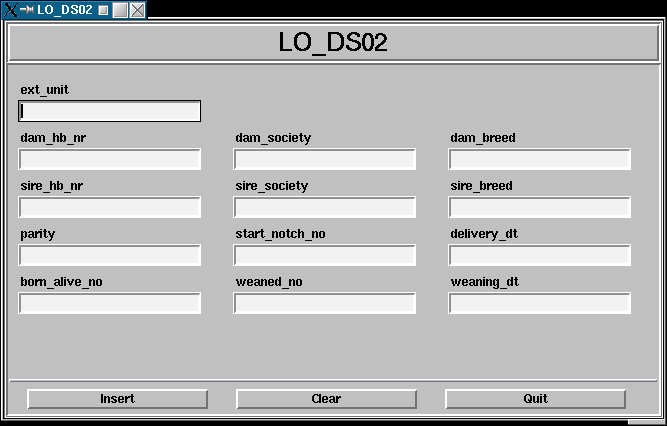
\includegraphics[%
  %  EG scale=0.4]{writing-LO/LO_DS02frm.png}
%  \end{center}
\end{figure}



